\section{Results and Analysis}
\label{analysis}

We analyze Mini-MAC for performance and security. 
Mini-MAC must be able to authenticate messages 
without compromising the performance of the real-time, safety-critical systems.

\subsection{Performance}
\label{performance}

Tables~\ref{tab-traffic}--\ref{tab-time} and Figures~\ref{fig-execution}--\ref{fig-ram}
show the message traffic, execution time, code size, and RAM usage of our unoptimized implementations
of Mini-MAC and their underlying HMACs.  Time and space are dominated by the HMAC computation.
Throughout, ``B''~denotes bytes, ``b''~denotes bits, and ``ms''~denotes milliseconds.

Table~\ref{tab-traffic} shows that Mini-MAC adds no additional bus traffic.
By contrast, HMAC-MD5 adds 128~bits (two CAN frames) per authentication,
due to the 128-bit tag.  Similarly, the pairwise-keyed Lin-MAC generates
two additional CAN frames per recipient ECU in each group communication.

Table~\ref{tab-time} shows the mean execution time
[what about standard deviation?] for each of our implementations of Mini-MAC.
Using MD5 is much faster than using SHA-1 or SHA-2.  As shown in Table~\ref{tab-overhead},
the overhead in time to compute Mini-MAC beyond HMAC is very little (approximately 0.38--0.68~ms).
Similarly, Figure~\ref{fig-execution} shows the mean execution times for Mini-MAC measured
in number of cycles on a 32~kHz clock.

Importantly, Table~\ref{tab-time} shows that only our MD5 implementtion of Mini-MAC runs fast enough to satisfy our
requirement of authenticating at least 40 messages per second (approximately
40~ms between messages).   
[check consistency of this calculation][also, explain why 28~ms for SHA-1 doesn't meet
this spec]
While highly optimized code might run faster, on the
basis of our timing measurements, we recommend implementing Mini-MAC using MD5.

Figure~\ref{fig-code} shows the code size of our Mini-MAC implementations.
As shown in Table~\ref{tab-overhead}, the additional code size for Mini-MAC beyond
HMAC is very small (approximately 800~bytes).

Figure~\ref{fig-ram} shows the RAM usage for our implementations of Mini-MAC.
As shown in Table~\ref{tab-overhead}, the overehead in RAM usage to compute Mini-MAC
beyond HMAC is very low (about 5~bytes).


%%% notes to me (ats)
%% be sure to comment on each of the issues from Section 6 (group keys, truncation, etc)

\subsection{Security}
\label{security}

	\begin{table*}	
	\centering
	\caption{Time-to-Defeat for Various Configurations}
	\label{tab-repeat}
	\vspace{8pt}
	\begin{tabular}{|l|c|r|r|r|}\hline%
	\bfseries Hash & \bfseries $\text{Counter}_{\text{R}}$ (b) & \bfseries $\text{Counter}_{\text{M}}$ (b) & \bfseries Msg. Before Repeat & \bfseries Min. Before Repeat\\\hline \csvreader[late after line=\\]%
		{tables/timetobeat.csv}{hash=\hash,rcounter=\rcounter,mcounter=\mcounter,msgbr=\msgbr,minbr=\minbr}% 
		{\hash & \rcounter & \mcounter & \msgbr & \minbr}%
		\hline
	\end{tabular}
	\end{table*}
	
Mini-MAC counters replay and masquerade attacks by forcing an attacker to wait a relatively long period of time before a MAC is repeated. Table 5 shows a comparision of the time-to-defeat (how long before the MACs are re-used) of the various hash bases and counter sizes. $R$ is the rollover counter size in bits, $M$ is the message counter size in bits, ``Msg BR" is the number of messages before repeat and ``Min BR" is the time in minutes before repeat at a data rate of 40 messages/second. This table (and Table 5) show the time-to-defeat for various configurations of Mini-MAC. This is the number of messages required before a MAC repeats multiplied by the maximum message rate per second.

%The table shows that most of these values (typically for message counter greater than or equal to 16 bits long) are sufficient for the automotive environment. 

The time to guess a 32-bit MAC correctly is much shorter than the time to repeat for most cases---only 27.3 minutes, on average, for an exhaustive search (brute force) guessing attack. This means that the most efficient use of resources is the smallest counter combination that withstands the time of a brute force attack. Therefore the 16-bit message counter is the best choice from the above because it will ensure a replay attack takes at least longer than the average time to execute a brute force attack on the MAC but will not consume more resources than is necessary.

The message data captured suggests an average message rate of approximately 25 messages/second. Some messages occur, however, at up to 40 messages/second, although this is unlikely. In the event that an attacker floods the system with a higher rate to cycle through the counters more quickly, ECUs on the bus could easily identify an illegitimate user. Figure 5 shows the probability density function of the time between messages. This relates the number of messages to defeat to a time-to-defeat figure by approximating how many messages per second an attacker can send.

%Mini-MAC also uses bus traffic history as well as a message counter and rollover counter to fend off replay attacks. The past five messages are stored by each ECU that has the authentication key for the message ID and these are used to transform the raw HMAC of the message. This transformation is then XORed with the message counter and processed through the HMAC algorithm. The rollover counter selects a starting bit in the resulting bit string and extracts the variable length MAC from this starting position. The message counter and rollover counters are both variable-length counters used to transform and select portions of the HMAC to be used as the transmitted MAC. The message counter ticks on every new message, and the rollover counter ticks on rollover of the message counter.

%While the length of the MAC is very short, it is more difficult to defeat with a replay attack than the length alone would suggest due to the use of the counter and message history. The counters ensure that the selected bits are not re-used, but the message history adds a non-deterministic amount of confusion to the message before the HMAC is even generated. To execute a replay attack, an attacker would have to wait for both counters to roll over  while at the same time the recent message history would have to perfectly align with a previously recorded value.

A key to Mini-MAC is that it uses the slow message rate of the CAN bus as an advantage. Malicious attackers must wait a long time (Table 4) to gain enough information to repeat a MAC. The use of message history in Mini-MAC ensures that even if an attacker has a long time to watch the bus, they will not be able to simply replay a message. It is worth noting as well that Table 4 shows the times for a stream of repeated messages, a case which is unlikely to repeat for the duration required to gain enough bits to repeat a MAC. Attackers cannot simply flood the network with messages designed to acquire responses more quickly because ECUs should be able to easily identify this behavior based on message delay statistics.

	\fontfamily{ptm}\selectfont
	\begin{figure}
		\centering
		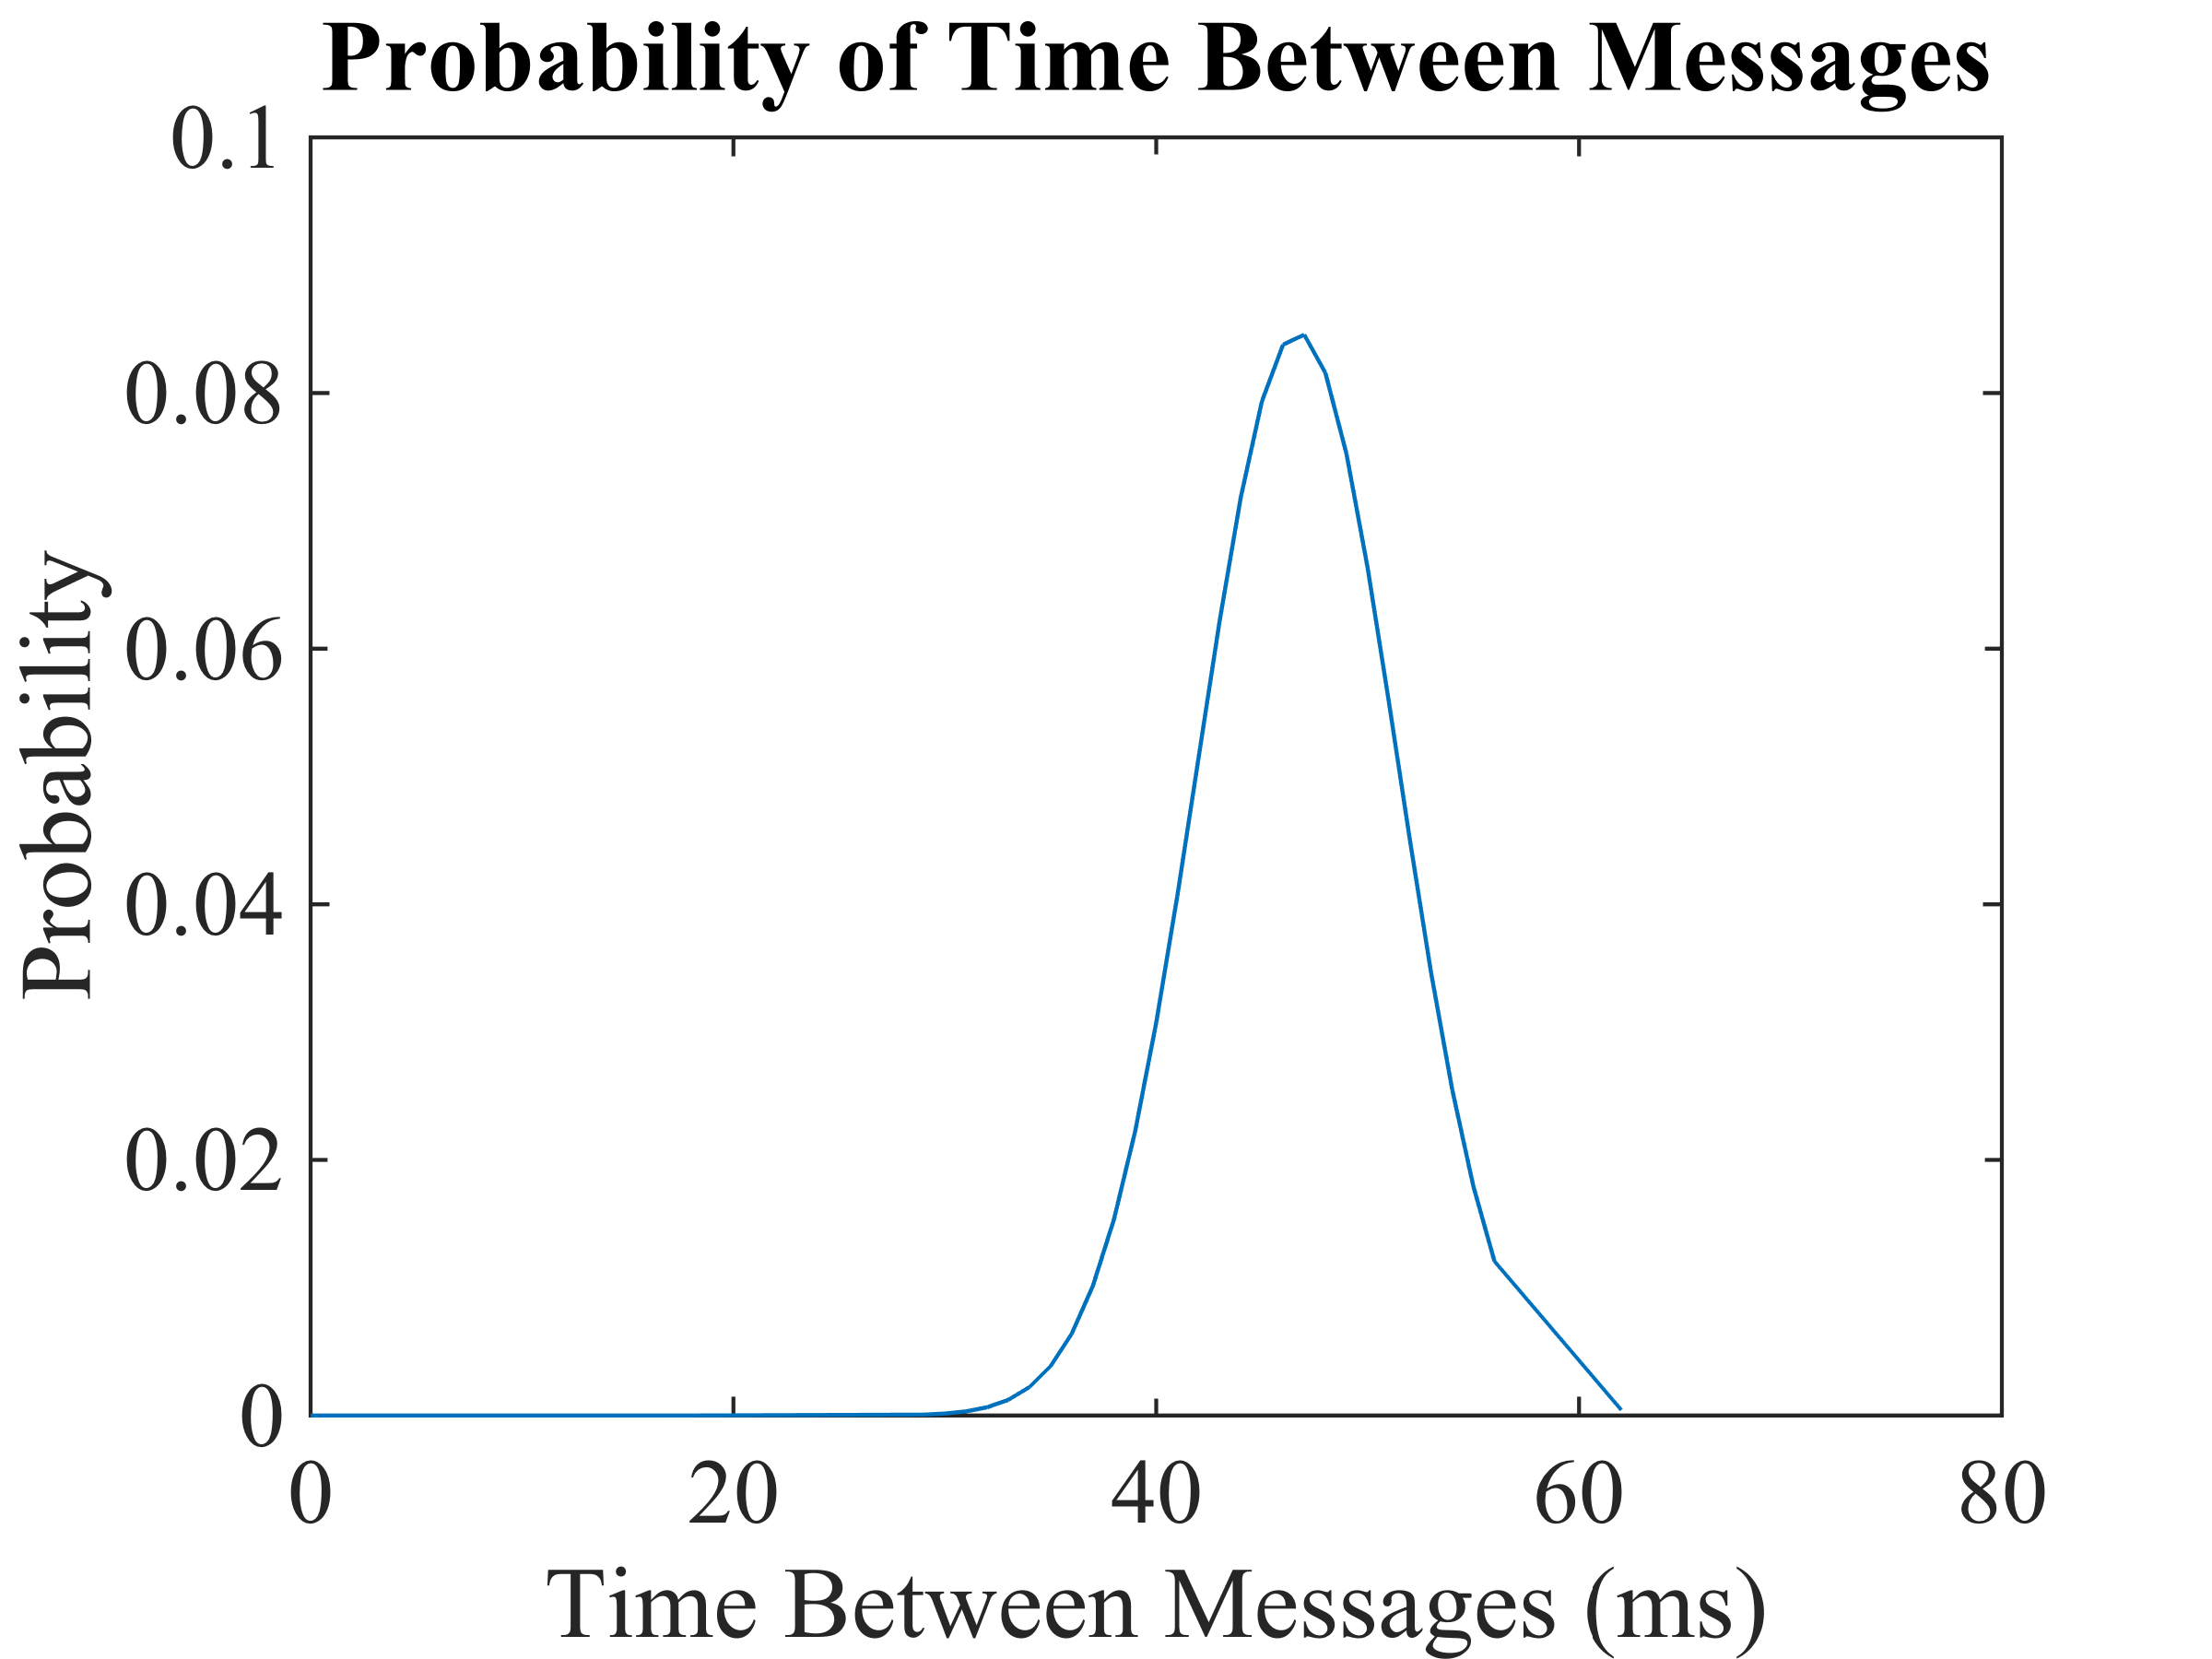
\includegraphics[width=\columnwidth]{figures/pdf.png}
		\caption{{\fontfamily{ptm}\selectfont Probability Density Function of Message Delay -- 
		ECUs can easily be able to identify nodes spamming messages}}
		\label{fig-msgdelay}
	\end{figure}
	
There are some attacks that will defeat Mini-MAC. Perhaps the easiest way to defeat any CAN security mechanism is by flooding the bus. The attacker does not need to try and break any security, but by preventing ECUs from talking to each other, the attack succeeds as the car will not be able to function properly. Similarly, if an ECU is flashed with corrupted firmware, it does not need the correct group keys to launch an attack. It needs only to wait long enough to see the counters roll over. Most people keep the same automobile for many years, so even if this attack requires several years to gather enough information, it will still eventually succeed. Mini-MAC is useful against a resourceful attacker, but not a patient one.
